\documentclass[12pt, openany]{report}
\usepackage[utf8]{inputenc}
\usepackage[T1]{fontenc}
\usepackage{amsmath,amsfonts,amssymb}
\usepackage{amssymb}
\usepackage{multicol}
\usepackage[a4paper,left=2.5cm,right=2.5cm,top=2.5cm,bottom=2.5cm]{geometry}
\usepackage[english]{babel}
\usepackage{libertine}
\usepackage{graphicx}
\usepackage{wrapfig}
\usepackage{float}
\usepackage{enumitem}
\usepackage{pythonhighlight}
\usepackage[]{titletoc}
\usepackage{empheq}
\usepackage{titlesec}
\usepackage{mathpazo}
\usepackage{xfrac}
\usepackage{textcomp}
\usepackage{mathtools}
\usepackage{caption}
\usepackage{tabularray}
\usepackage{subcaption}
\usepackage[bottom]{footmisc}
\usepackage{pdfpages}
\usepackage{tabularx}
\usepackage[skins]{tcolorbox}
\titleformat{\chapter}[display]
  {\normalfont\bfseries}{}{0pt}{\Huge}
\usepackage{hyperref}
\newcommand{\hsp}{\hspace{20pt}}
\newcommand{\HRule}{\rule{\linewidth}{0.5mm}}
\newcommand\independent{\protect\mathpalette{\protect\independenT}{\perp}}
\def\independenT#1#2{\mathrel{\rlap{$#1#2$}\mkern2mu{#1#2}}}

% Define a new tcolorbox style with a red border and transparent interior
\tcbset{
    redbox/.style={
        enhanced,
        colframe=red,
        colback=white,
        boxrule=1pt,
        sharp corners,
        before skip=10pt,
        after skip=10pt,
        box align=center,
        width=\linewidth-2pt, % Adjust the width dynamically
    }
}
\newcommand{\boxedeq}[1]{
\begin{tcolorbox}[redbox]
    \begin{align}
        #1
    \end{align}
\end{tcolorbox}
}

\begin{document}


\begin{titlepage}
    \begin{sffamily}
    \begin{center}
        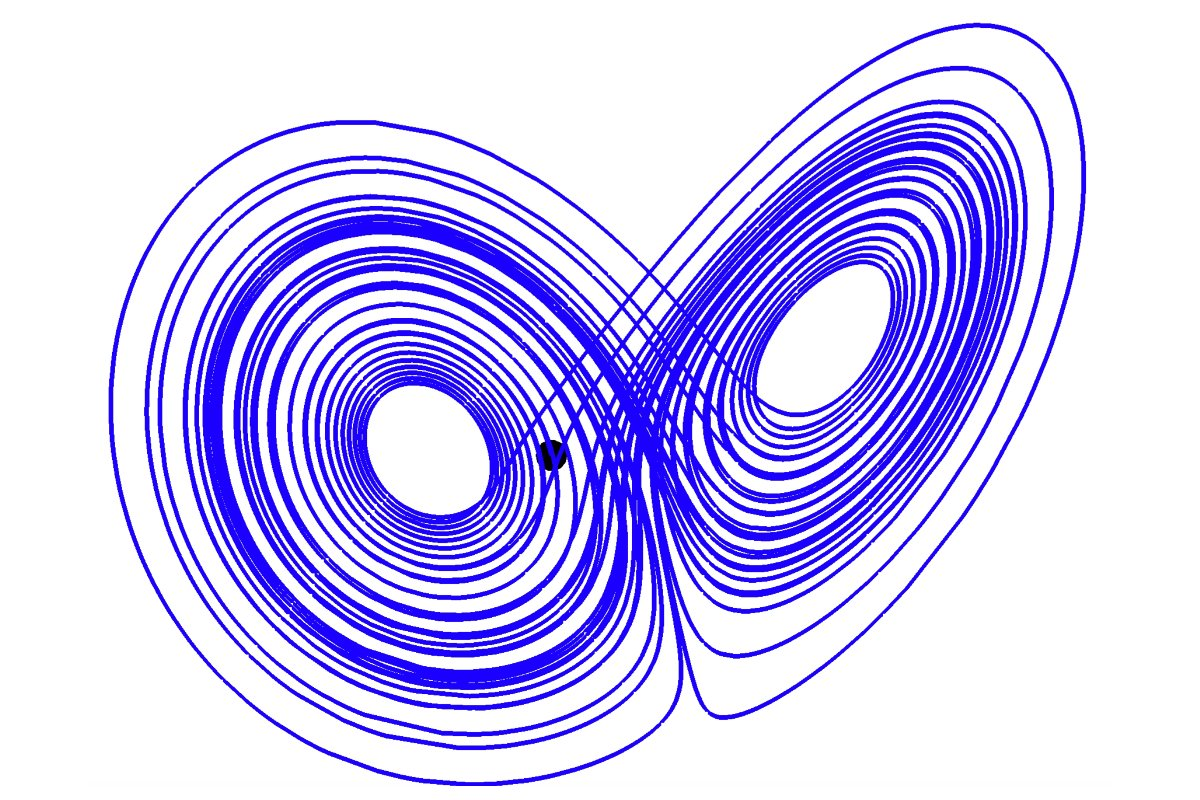
\includegraphics[scale=0.25]{img/page_de_garde.png} \\[1cm]
        \HRule \\[0.4cm]
        { \huge \bfseries LINMA2370 Modelling and Analysis of Dynamical Systems \\[0.4cm] }
    
        \HRule \\[1.5cm]
        \textsc{\LARGE Simon Desmidt\\Issambre L'Hermite Dumont}\\[1cm]
        \vfill
        \vspace{2cm}
        {\large Academic year 2024-2025 - Q1}
        \vspace{0.4cm}
         
        
\includegraphics[width=0.15\textwidth]{img/epl.png}
        
        UCLouvain\\
    
    \end{center}
    \end{sffamily}
\end{titlepage}

\setcounter{tocdepth}{1}
\tableofcontents

% \chapter{Methodology}

% \section{Theoretically}
% The modelisation and the analysis of a dynamical system requires to follow a set of steps, in order to have a clear overview of the system.\\

% Firstly, we can draw the system that we want to model, at rest and in the movement that we want to analyse.\\

% After that, we will model the system and its dynamics with a set of ODE.\\

% And finally, we can analyse the system and its modelisation, in order to understand it. For example we can analyse the quantitive and qualitative behaviour of the system. Its equilibrium point(s), and the eigenvalues of the problems that will show the mode/focus where the system tends to.\\
% Steps to follow, in order to have an overview of the system:
% \begin{itemize}
%     \item draw the system at rest/in useful mvt
%     \item model the system with ODE's
%     \item solve ODE system
%     \item analyse the eigenvalues and how the system reacts
%     \item deduce a qualitative/quantitative behaviour of the system
% \end{itemize}

% \section{Example}
% Tacoma Narrows Bridge

% \chapter{Terminology and notation}

\chapter{Introduction}
The tools introduced in this course are a simplifying view of the reality, yet very uselful to build simple and effective models in view of the control and optimization of the dynamical behaviour of the real systems.
\section{Reminders}
\begin{itemize}
    \item A subset of \(\mathbb{R}\) is said to be negligible if its Lebesgue measure is equal to zeroo and that a property is said to be true almost everywhere if it is false only on a negligible set. 
    \item Let \(I\subseteq \mathbb{R}\) be an interval the interior of which is not empty. A function \(x:I\rightarrow \mathbb{R}^N\) is said to be absolutely continuous if 
\end{itemize}
\begin{multline*}
        \forall \varepsilon \in (0,\infty),\: \exists \delta\in (0,\infty) \: : \\
        \forall n\in \mathbb{N}\setminus\{0\},\: \forall a_1,b_1,\dots, a_n,b_n\in I : \\ 
        a_i<b_i \: \forall i\in \{1,\dots,n\}, \: b_i\le a_{i+1} \:\forall i\in \{1,\dots,n-1\}, \\
        \sum_{i=1}^n(b_i-a_i)\le \delta \Longrightarrow \sum_{i=1}^n \lVert x(b_i)-x(a_i)\rVert \le \varepsilon
\end{multline*}
\begin{itemize}
    \item Let \(a,b\in \mathbb{R}\) with \(a<b\). A function \(x:[a,b]\rightarrow \mathbb{R}\) is absolutely continuous iff there exists an integrable fucntion \(\varphi:[a,b]\rightarrow \mathbb{R}\) such that, for every \(t\in [a,b]\), \[x(t) = x(a0) + \int_a^t \phi(s)ds\] in which case \(x\) is almost everywhere differentiable with \(\dot x(t) = \phi(t)\) for almost every \(t\in [a,b]\). 
    \item A function \(f:\Omega\rightarrow \mathbb{R}^N\), where \(\Omega\) is a nonempty subset of \(\mathbb{R}\times \mathbb{R}^N\), is said to be Lipschitz continuous in the second argument, uniformly with respect to the first argument, if there exists \(L\in \left[0,\infty\right)\) such that forall \(t\in \mathbb{R}\) and all \(x,y\in \mathbb{R}^N\) such that \((tx,),(t,y)\in \Omega\), \[\lVert f(t,x)-f(t,y)\rVert \le L\lVert x-y\rVert\] It is said to be locally Lipschitz continuous on an open ball for each argument. 
    \item Let \(\Omega\) be a nonempty open subset of \(\mathbb{R}\times \mathbb{R}^N\) and \(f:\Omega\rightarrow \mathbb{R}^N\) be such that 
    \begin{itemize}
        \item for all \(t\in \mathbb{R},\: f(t,\cdot):\Omega_t\rightarrow \mathbb{R}^N\)
        \item \(\partial_2f:\Omega \rightarrow \mathcal{L}(\mathbb{R}^N,\mathbb{R}^N):(t,x)\rightarrow \partial_2f(t,x)\) is locally bounded.
    \end{itemize}
\end{itemize}
Then, \(f\) is locally Lipschitz continuous in the second argument, uniformly with respect to the first argument.
\begin{itemize}
    \item If \((X,\lVert \cdot \rVert_X)\) and \((Y,\lVert \cdot \rVert_Y)\) are two real normed spaces, and the real vector space \(\mathcal{L}(X,Y)\) of all continuous linear mappings from \(X\) to \(Y\)\footnote{Meaning matrix from \(X\) to \(Y\)} is equipped with the norm defined by \[\lVert L\rVert \coloneqq \sup_{x\in X\setminus\{0\}}\frac{\lVert Lx\rVert_Y}{\lVert x\rVert_X}\]
\end{itemize}
\section{State-space model}
A state-space model for a continuous dynamical system consists of an ODE of the form 
\begin{equation}\label{eq:1}
    \dot x (t) = f(t,x(t))
\end{equation}
where the function \(f:\Omega\rightarrow \mathbb{R}^N\), \(\Omega\) being a nonempty subset of \(\mathbb{R}\times \\mathbb{R}^N\), is called the vector field associated with the ODE.
A continuous dynamical system with input \(u:\mathbb{R}\rightarrow \mathbb{R}^M\) described by the ODE 
\begin{equation}
    \dot x(t) = g(x(t),u(t))
\end{equation}
for some function \(g:\mathbb{R}^N\times \mathbb{R}^M\rightarrow \mathbb{R}^N\), can be written in the form \ref{eq:1} by defining the vector field \
\begin{equation}
    f_u :\mathbb{R}\times \mathbb{R}^N \rightarrow \mathbb{R}^N :(t,x) \rightarrow g(x,u(t))
\end{equation}
\begin{itemize}
    \item [\(\rightarrow\)] N.B.: the norm of each \((t,x)\in \mathbb{R}\times \mathbb{R}^N\)  is defined as \(|t|+\lVert x\rVert\).
\end{itemize}
\section{Integral curve}
Let \(\Omega\) be a nonempty subset of \(\mathbb{R}\times \mathbb{R}^N\). An integral curve of \(f:\Omega\rightarrow \mathbb{R}^N\) is a function \(x:I\rightarrow \mathbb{R}^N\) where \(I\subseteq \mathbb{R}\) is an interval, for which the interior is not empty, called the interval of existence of \(x\), i.e. differentiable and satisfies \((t,x(t))\in \Omega\) and \(\dot x(t) = f(t,x(t))\) for all \(t\in I\). The graph \(\{(t,x(t))|t\in I\}\) and the image \(\{x(t)|t\in I\}\) of \(x\) are respectively called the trajectory and the orbit of \(x\). Given an initial condition \((t_0,x_0)\in \Omega\), a solution to the initial value problem 
\begin{equation}
    \begin{cases}
        \dot x(t) = f(t,x(t))\\
        x(t_0) = x_0\\
    \end{cases}
\end{equation}
is an integral curve \(x:I\rightarrow \mathbb{R}^N\) of \(f\) such that \(t_0\in I\) and \(x(t_0)=x_0\). \\

If, for the IVP described hereabove, \(f\) is continuous, then a continuous function \(x:I\rightarrow \mathbb{R}^N\) where \(I\subseteq \mathbb{R}\) is an interval containing \(t_0\) and the interior of which is not empty, is a solution iff its graph is contained in \(\Omega\) and it satisfies the integral equation \[x(t)=x_0+\int_{t_0}^tf(s,x(s))ds\] for all \(t\in I\). In that case, \(\dot x\) is continuous. \\

Let \(\Omega\) be a nonempty subset of \(\mathbb{R}\times \mathbb{R}^N\). An integral curve in the extended sense of \(f:\Omega\rightarrow \mathbb{R}^N\) is a function \(x:I\rightarrow \mathbb{R}^N\), where \(I\subseteq \mathbb{R}\) is an interval the interior of which is not empty called the interval of existence of \(x\), that is absolutely continuous and satisfies \((t,x(t))\in \Omega\) for every \(t\in I\) and \(\dot x(t) = f(t(x(t)))\) for almost every \(t\in I\). 
\begin{itemize}
    \item [\(\rightarrow\)] N.B.: If \(f\) is continuous, then the two definitions of integral curves are equivalent.
\end{itemize}
\section{Existence of a solution}
Consider the IVP defined hereabove with an integral curve in the extended sense, under the following assumptions:
\begin{itemize}
    \item there exists \(\tau,r\in (0,\infty)\), such that \([t_0-\tau,t_0+\tau]\times B(x_0,r)\subseteq \Omega\);
    \item for every \(x\in B(x_0,r)\), the function \([t_0-\tau,t_0+\tau]\rightarrow \mathbb{R}^N:t\rightarrow f(t,x)\) is measurable;
    \item for every \(t\in [t_0-\tau,t_0+\tau]\), the function \(B(x_0,r)\rightarrow \mathbb{R}^N:x\rightarrow f(t,x)\) is continuous;
    \item there exists an integrable function \(m:[t_0-\tau,t_0+\tau]\rightarrow \left[0,\infty\right)\) such that \[\lVert f(t,x)\rVert \le m(t) \text{ for all }(t,x) \in [t_0-\tau,t_0\tau]\times B[x_0,r]\]
\end{itemize}
Then, there exists a solution defined on a compact interval the interior of which contains \(t_0\). \\
In particular, for the IVP with an integral curve in the general sense, if \((t_0,x_0)\) is an interior point of \(\Omega\) and \(f\) is continuous, then there exists a solution defined on a compact interval the interior of which contains \(t_0\).
\chapter{Dynamical systems and state-space models}
We will study first-order dynamical systems of the form 
\begin{equation}\label{eq:ODE}
    \dot x = f(x,u)
\end{equation}
where \(f\) is a mapping from \(\mathbb{R}^{n+m}\) to \(\mathbb{R}^n\), while \(x\) and \(u\) are vector functions of time, respectively the state and the input. 
\section{Terminology and notation}
\begin{itemize}
    \item We assume that the input is a piecewise continuous and bounded function: \(u\in \mathcal{U}\), where \(\mathcal{U}\) is a set of piecewise continuous and bounded functions from \(\mathbb{R}\) to \(\mathbb{R}^m\).
    \item For a given value of the initial state \(x(t_0)=x_0\) a,d a given input \(u\), the solution \(t\rightarrow x(t)\) for \(t\ge t_0\), of the system of ODE \ref{eq:ODE} is called the trajectory of the system. It is denoted \(x(t_0,x_0,u)\).
    \item When the input \(u\) can be freely chosen in \(\mathcal{U}\), the system \(\dot x = f(x,u)\) is said to be a forced/controlled system. 
    \item [\(\rightarrow\)] N.B.: in this course, we will study the solution of the equation \ref{eq:ODE} when the input is actually an a priori set constant: \(u(t) = \overline{u}\) \(\forall t\ge t_0\). The state-space model is then written as \(\dot x = f(x,\overline{u}) = f_{\overline{u}}(x)\).
\end{itemize}
\subsection{System with affine input}
\begin{equation}
    \dot x = f(x) + \sum_{i=1}^m u_ig_i = f(x) + G(x)u
\end{equation}
where \(f\) and \(g_i\) are mappings from \(\mathbb{R}^n\) to \(\mathbb{R}^n\). 
\subsection{System with affine state}
\begin{equation}
    \dot x = \sum_{i=1}^n x_ia_i(u) + b(u) = A(u)x+b(u)
\end{equation}
where \(b\) and \(a_i\) are mappings from \(\mathbb{R}^m\) to \(\mathbb{R}^n\). 
\subsection{Bilinear systems}
A bilinear system is affine both in the state and in the input:
\begin{equation}
    \dot x = \left(A_0 + \sum_{i=1}^mu_iA_i\right) x + B_0u 
\end{equation}
where \(A_i\) and \(B_i\) are matrices of dimensions \(n\times n\) and \(n\times m\) respectively. 
\subsection{Linear system}
\begin{equation}
    \dot x = Ax + Bu
\end{equation}
where \(A\) and \(B\) are matrices of dimensions \(n\times n\) and \(n\times m\) respectively. 
\end{document}